%\documentclass{article}
%\usepackage[a4paper, total={6in, 8in}]{geometry}
\documentclass[reprint,amsmath,amssymb,rmp,onecolumn,notitlepage,11pt]{revtex4-1}
\usepackage[utf8]{inputenc}
%\usepackage{authblk}
%\usepackage{natbib}
\usepackage[normalem]{ulem}
\usepackage{graphicx}
\usepackage{hyperref}
\usepackage{xcolor}
\newcommand{\red}[1]{\textcolor{red!80!black}{#1}}
\newcommand{\blue}[1]{\textcolor{blue!80!black}{#1}}
\newcommand{\green}[1]{\textcolor{green!70!black}{#1}}
\usepackage{mathtools}
\DeclarePairedDelimiter{\evdel}{\langle}{\rangle}

\begin{document}
\title{Linklength distribution in Proteins and our model}
\title{The role of geometry in the chain separation distribution of links in protein contact networks}
%\title{}
%\title{}
%\title{}
\author{Antonia Mey}
\affiliation{EaStCHEM School of Chemistry, University of Edinburgh, Edinburgh, United Kingdom}
\author{Steffen Mühle}
\affiliation{Uni Göttingen, 37077 Göttingen, Germany}
\author{Nora Molkenthin}
\email[Electronic Address: ]{n.molkenthin@gmx.de}
\affiliation{Potsdam Institut für Klimafolgenforschung, Potsdam, Germany}
\affiliation{Chair for Network Dynamics, Institute for Theoretical Physics and Center for Advancing Electronics Dresden (cfaed), Technical University of Dresden, 01069 Dresden}
%\author{Marc Timme}
% \affiliation{Network Dynamics, Max Planck Institute for Dynamics and Self-Organization (MPIDS), 37077 Göttingen, Germany}
% \affiliation{Chair for Network Dynamics, Institute for Theoretical Physics and Center for Advancing Electronics Dresden (cfaed), Technical University of Dresden, 01069 Dresden}

\begin{abstract}
The distribution of chain separations of interacting amino acids in proteins roughly follows a power law. Here we show, analytically and in simulations, that a geometrical stochastic model of folding chains can explain this behaviour. %Separating the data in $\alpha$-dominated, $\beta$-dominated and intrinsically disordered proteins (IDP's) shows characteristic structures in the distribution due to the secondary structure.
\end{abstract}
\maketitle

\section*{Introduction}
\begin{enumerate}
    \item Proteins are very important \cite{a bunch of stuff}
    \item Proteins can be modeled as networks of amino acids and their connections \cite{Vendruscolo2002,DiPaola2013,Estrada2011}.
    \item They postulate/observe that proteins have a sequence separation distribution, that is 1/l in \cite{bartoli2008effect}.
    \item Here we explain this from geometric constraints alone using a model introduced in \cite{Molkenthin2016,molkenthin2020self}
\end{enumerate}
TO DO: Write text
\section*{Model}
\begin{enumerate}
    \item Model in General
    \item Simplified 2D version
\end{enumerate}
TO DO: Write text
\section*{Analytic approximation}
Starting from a closed chain of $N$ unit discs, as introduced for the analytic calculations in \cite{molkenthin2016scaling}.
Let us start by introducing the auxiliary variable $F(s)$, defined to be the number of possible links with a sequence separation of $s$. Before any links are added all sequence separations are equally likely, as there are $N$ possibilities of making a link of each separation $s$ with $2\leq s < N/2$.

As we add more links, not only are links taken out of this pool, because they have already been realized, each existing link can also geometrically prohibit other connections.
Let us call the poos of available links after $i$ links have been added $F_i(s)$.

-------------- Add Figure explaining which links are geometrically excluded --------------

The expected distribution of possible links after one step is given by the average over available link pools taken over all possible lengths of the initial link
\begin{equation}
    F_1(s)= \frac{1}{N/2-2} \sum_{s_1=2}^{N/2} { \begin{cases}
    N-2(s-1) \text{ , for } s<s_1\\
    N-2(s_1 -1)\text{ , for } s\geq s_1
    \end{cases}}.
\end{equation}

In subsequent steps we get the same reduction but starting from the pool of the step before rather than the full $N$ links for each length, leading to an additional probability factor 
\begin{equation}
    P_k(s)=\frac{F_k(s)}{C_k},
    \label{eq.Pk}
\end{equation}
with $C_k=\sum_{s=2}^{N/2}F^k(s)$, for each segment separation $s$ to occur and thus
\begin{equation}
    F_k(s)= \frac{1}{N/2-2} \sum_{s_k=2}^{N/2} {\begin{cases}
     F_{k-1}(s)-2(s-1) P^k(s) \text{ , for } s<s_k\\
     F_{k-1}(s)-2(s_k -1)P^k(s)\text{ , for } s\geq s_k
    \end{cases}}.
\end{equation}
This can be simplified to 
\begin{align}
   F_k(s)&= \frac{1}{N/2-2} \frac{F_{k-1}(s)}{C_{k-1}}\left( \sum_{s_k=2}^{N/2}C_{k-1} - \sum_{s_k=2}^{s} 2(s-1) - \sum_{s_k=s+1}^{N/2} 2(s_k -1) \right) \nonumber \\
   &= \frac{1}{N/2-2}\frac{F_{k-1}(s)}{C_{k-1}}\left((N/2-2)C_{k-1}- 2(N/2-(s+1))(s-1) - ((s-1)(s+1))\right)  \nonumber \\
   &=F_{k-1}(s)\left(1-\frac{f(s)}{(N/2-2)C_{k-1}} \right)
   \label{eq.Fk_rec}
\end{align}
Where we defined $f(s)=2(N/2-(s+1))(s-1) + ((s-1)(s+1))$ for notational brevity. \red{Maybe we can try to simplify this expression some more.}

We can now use the recursive expression Eq.~\ref{eq.Fk_rec} to write down a closed expression for $F_k(s)$

\begin{equation}
    F_k(s)=N\prod_{i}^k\left(1-\frac{f(s)}{(N/2-2)C_{k-1}} \right)
\end{equation}

The probability distribution of the realized sequence separations of all added links is then given by the average over the available pools at each link addition step, leading to
\begin{align}
    P(s)&=\frac{1}{N-3}\sum_{k=0}^{N-3} P_k(s) \nonumber \\
    &= \frac{N}{N-3}\sum_{k=0}^{N-3} \frac{1}{C_k}\prod_{i}^k\left(1-\frac{f(s)}{(N/2-2)C_{k-1}} \right),
\end{align}
which makes use of Eq.~\ref{eq.Pk}. The only unknown in this expression is $C_k$, which we can not compute exactly. However, since $C_k$ monotonically decreases with $k$, $N>C_k>C_{N-2}$ always holds and we can obtain an upper and lower bound by replacing all $C_k$ in the expression with either $N$ (underestimates all probabilities) or $C_{N-2}$ (overestimates all probabilities). Each time we get an expression of the form 
\begin{align}
     P(s)&\approx\frac{N}{N-3}\frac{1}{C}\sum_{k=0}^{N-3} \prod_{i}^k\left(1-\frac{f(s)}{(N/2-2)C} \right)\nonumber \\
     &=\frac{N}{N-3}\frac{1}{C} \frac{1}{\alpha s}.
\end{align}
Here we have made use of the geometric series and made the substitution $1-\frac{f(s)}{(N/2-2)C} = 1- \alpha s $.

\red{ah, I forgot to copy down why $f(s)$ is linear in s, which is kind of crucial for this argument, it's in my notes somewhere.}

\red{is that plausible? I guess if the difference of $N$ and $C_{N-2}$ is large that leaves quite a large range...}

\section*{Data and simulations}
\begin{enumerate}
    \item Show plots of distribution for data, simulation and analytics
    \item Maybe comment on chin length dependence
    \item Look into the dip we saw there once
\end{enumerate}
\begin{figure}[h]
        \centering
	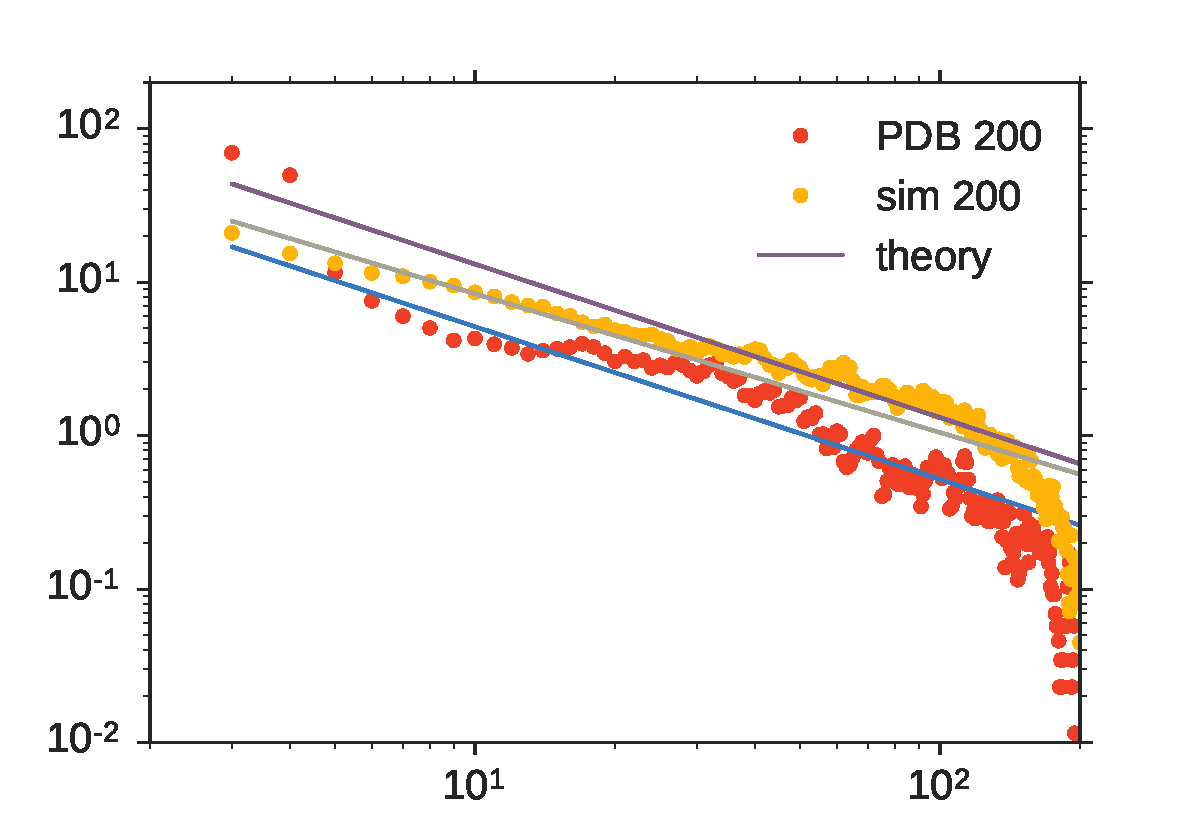
\includegraphics[width=0.45\textwidth]{both_dist_200.pdf}
	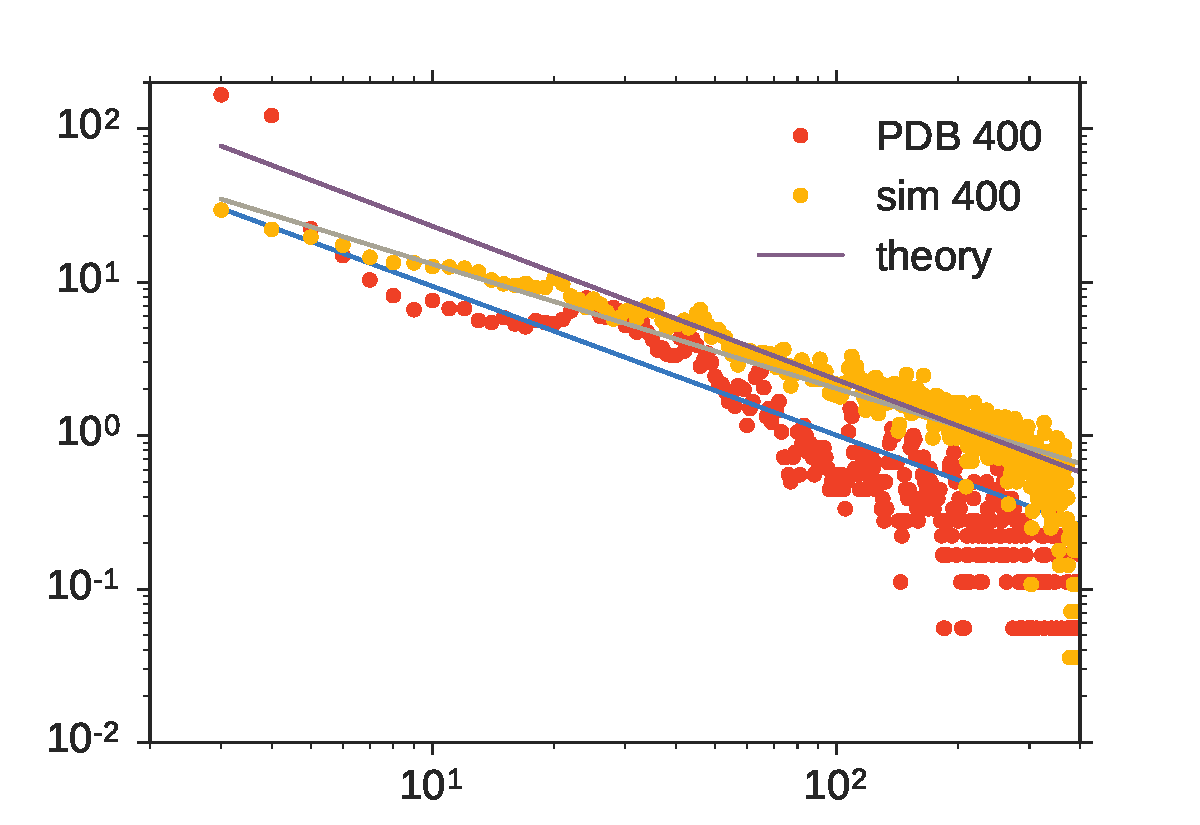
\includegraphics[width=0.45\textwidth]{both_dist_400.pdf}
        \caption{New figure is averaged over more structures (no alpha beta selection), need to explain why the rule only works for link lengths between 20 and N/2. Or why there is a bump, it seems more like a bump than a dip now...
        }
        \label{fig:time_scaling}
\end{figure}
\section*{Conclusion}
\begin{enumerate}
    \item We can now explain the sequence separation from geometry and even do it analytically.
    \item Maybe something about helixes and sheets and the dip.
\end{enumerate}
TO DO: Leave until the rest is done.
\section*{Declarations}
\subsection{Availability of data and materials}
All data generated or analysed during this study are included in this published article [and its supplementary information files].
\subsection{Competing interests}
The authors declare no competing interests.
\subsection{Funding}
This research was supported by ...
\subsection{Authors' contributions}

\subsection{Acknowledgements}
We thank ... for fruitful discussions.

\bibliographystyle{unsrt}
\bibliography{proteins}

\appendix
\section{Supplemental Material Collection}
\section{Random ideas}
\begin{itemize}
    \item Why is the beginning different for simulations?
    \item Does the dip disappear for IDPs
    \item Can we use all NMR structures for IDPs
    \item Would it help using more simulated structures than just the Crystal structure. 
\end{itemize}
TODO: @Toni: Collect data and plotting scripts in github
TODO: @Toni: Connect overleaf to github


\end{document}